%\documentclass[a4paper,]{book}
\documentclass[a4paper, twoside,openright ,titlepage, 12pt]{book}
\usepackage[english]{babel}
\usepackage{preamble}
\usepackage[MEK,60]{masterfrontpage}
\setlength\parindent{0pt}
\begin{document}
\masterfrontpage	
\maketitle

\pagenumbering{roman}
\tableofcontents
\newtheorem{theorem}{Theorem}[section]
\newtheorem{lemma}[theorem]{Lemma}
\pagenumbering{arabic}
%\chapter{A motivation for studying fluid-structure interaction}
The interaction between fluid and solids can be observed all around us in nature and has shown crucial in engineering. Examples in nature include swimming fish, flying birds, or trees bending in the wind. Man has learned from nature and has traditionally relied upon laboratory experiments to design windmills, aircrafts, and bridges. The importance of understanding fluid-structure (or solids) interaction (FSI) cannot be overstated, as the lack of such has demonstrated to be disastrous in the design of everything from bridges to airplanes. Let alone to emphasize our incapability to replicate the performance of nature; we're far away from designing a drone capable of flying like a hummingbird. However, laboratory experiments are inherently noisy, expensive, and results can be difficult to reproduce. A much cheaper and indeed smarter approach to studying FSI is using computers, or more specifically numerical simulations to gain fundamental insight to the interaction between fluids and solids. The latter has on the other hand shown to be difficult to realize, for a number of reasons related to both mathematical and computational reasons. Therefore, the goal of this thesis is to develop an open-source framework using standard techniques for solving FSI problems that can be used as a point of reference for future benchmarking of FEniCS-based FSI solvers. \\

The main goal of this thesis is to create a verified and validated monolithic fluid-structure interaction solver in FEniCS, which can handle large deformations. To achieve this, I have defined four subgoals: 

\begin{itemize}
\item Formulate a weak variation for a monolithic arbitrary Lagrangian Eulerian fluid-structure interaction problem.
\item Construct a finite element solver for the fluid-structure interaction problem.
\item Verify and validate a finite element solver for the fluid-structure interaction problem.
\item Compare the impact of discretization and mesh lifting operators on the final solution.
\item Improve computational efficiency of the implementation.
\end{itemize}


Each of the following subgoals will be addressed in separate chapters organized as follows: Balance of linear momentum for both solids and fluids are first introduced together with conservation of mass. The Eulerian, Lagrangian, and the arbitrary Lagrangian-Eulerian (ALE) frames of reference are briefly introduced to express the governing equations, before the equations describing FSI are derived. The numerical implementation is verified using the most rigorous convergence tests, before validation is performed against state-of-the-art benchmarks. Finally, computational speed-up is addressed together with long-term numerical stability of the coupled problem, and methods to overcome these challenges.
 

%\newpage
%\chapter{Continuum Mechanics}
When studying the dynamics of a mediums with fluid or structure properties under the influence of forces, we need in some sense a good description of how these forces act and alter the system itself.

Any medium on a microscopic scale is built up of a structure of atoms, meaning we can observe "empty spaces " between each atom or discontinuities in the medium. Discribing any phsycial phenomen on larger scales in such a way are tedious and most often out of bounds due to the high number of particles. Instead we consider the medium to be continously distributed throughout the entire reagion it occupies. Hence we want to study some phsyical properties of the complete volume and not down on atomic scale. 

We consider the medium with continuum properties. By a continuum we mean a volume $V(t) \subset \mathbb{R}^3$ 
consiting of particles, which we observe for some properties. One property of interest could be the veloctity $\textbf{v}(x,t)$ for some point $x \in V(t)$ in time $t \in (0, T]$, which would mean the average velocity of the particles occupying this point \textit{x} at time \textit{t}  

\section{Coordinate system}
We assume that our medium is continiously distributed throughout its own volume, and we start our observation of this medium
at som time $t_0$. As this choice is arbitary, we often choose to observe a medium in a stress free initial state. We call this state $V(t_0)$ of the medium as the \textit{reference configuration}. We let $V(t)$ for 
$t \geq t_0$ denote the \textit{current configuration}. \\ \\

\subsection{Lagrangian}
As the medium is act upon by forces, one of the main properties of interest is the deformation. Let \^{x} be a particle in the reference cofiguration $\ha{x} \in \ha{V}$. 
Further let x(\^x, t) be the new location of a particle \^x for time t such that $x \in V(t)$. We assume that no two particles $\ha{x}_a, \ha{x}_b \in \ha{V}$ occupy the same location for some time $V(t)$.
Hence the map $\ha{T}(\ha{x}, t) = x(\ha{x}, t)$ maps a particle \ha{x} from the \textit{reference configuration} $\ha{V}$ to the  \textit{current configuration} $V(t)$
Assuming that the path for some \^{x} is continious in time, we can define the inverse mapping $\ha{T}^{-1}(x, t) = \ha{x}(x, t)$, which maps $x(\ha{x}, t)$ back to its initial location at time $t = t_0$. \\

We now have enough background to define the \textit{deformation} 
\begin{align}
\hat{u}(\ha{x},t) = x(\ha{x},t) - \ha{x} 
\end{align}

and the \textit{deformation velocity}
\begin{align}
\hat{v}(\ha{x},t) = d_t x(\ha{x},t) = d_t \hat{u}(\ha{x},t) 
\end{align}

Such a description of tracking each particle $\ha{x} \in \ha{V}$ is often denoted the \textit{Lagrangian Framework} and is a natural choice of describing structure mechanics.
\subsection{Eulerian}
Considering a flow of fluid particles in a river, a \textit{Lagrangian} description of the particles would be tidious as the number of particles entring and leaving the domain quickly rise to a immense number. 
Instead consider defining a view-point $V$ fixed in time, and monitor every fluid particle passing the coordinate $x \in V(t)$ as time elapses. Such a description is defined as the \textit{Eulerian framework.} 
It is important to mention that the we are not interested in which particle is occupying a certain point in our domain, but only its properties. Such a description falls natural for describing fluid dynamics. \\
We can describe the particles occupying the \textit{current configuration} $V(t)$ for some time $t \geq t_0$ 
\begin{align*}
x = \ha{x} + \hat{u}(\ha{x}, t)	
\end{align*}
Since our domain is fixed can define the deformation for a particle 
occupying position $x = x(\ha{x},t)$ as
\begin{align*}
\textbf{u}(x, t) = \hat{u}(\ha{x}, t) = x - \ha{x}	\\
\end{align*}
and its velocity
\begin{align*}
\textbf{v}(x,t) = \partial_t u(x,t) = \partial_t \hat{u}(\ha{x},t) = \hat{v}(\ha{x},t)
\end{align*}

\section{Deformation gradients}
When studying continuum mechanics we observe continious mediums as they are deformed over time. These deformations
results in relative changes of positions due to external and internal forces acting.. These relative changes of postition is called
\textit{strain}, and is the primary property that causes \textit{stress} within a medium of interest \cite{Richter2016}. We define stress as the internal forces that particles within a continuous material exert on each other. \\

The equations of mechanics can be derived with respect to either a deformed or undeformend configuration of our medium of interest. The choice of refering our equations to the current or reference configuration is indifferent from a theoretical point of view. In practice however this choice can have a severe impact on our strategy of solution methods and physical of modelling.   \cite{Wriggers2006}. We will therefore define the strain measures for both configurations of our medium.  

\begin{defn}
Deformation gradient. 
\begin{align}
\hat{F} = I + \hat{\nabla} \hat{u} 
\end{align} 
\end{defn}

Mind that deformation gradient of $\ha{u}$ is which respect to the reference configuration. 
From the assumption that no two particles $\ha{x}_a, \ha{x}_b \in \ha{V}$ occupy the same location for some time $V(t)$, the presented transformation must be linear. As a consequence from the invertible matrix theorem found in linear algebra, the linear operator \textbf{F} cannot be a singuar.  
We define the  \textit{determinant of the deformation gradient} as \textit{J}, which denotes the local change of volume of our domain. 

\begin{defn}
Determinant of the deformation gradient
\begin{align}
J = det(\hat{F}) = det( I + \hat{\nabla} \hat{u} ) \neq 0
\end{align} 
\end{defn}


By the assumption that the medium can't be selfpenetrated, we must limit  J to be greater than 0 \cite{Wriggers2006}


\section{Transformations}
The deformation gradient and the determinant of the deformation gradient are central properties transforming line, area and volume elements between the reference and current configurations.   We have
\begin{align*}
&\text{Line element} \hspace{6mm}\int_{V(t)} dx = \int_{\ha{V}} \hat{F} d\ha{x} \\
&\text{Area element} \hspace{6mm}\int_{V(t)} \textbf{n } da = \int_{\ha{V}} J\hat{F}^{-T} \textbf{n} \hspace{2mm} d\ha{x} \\
&\text{Volume element} \hspace{2mm} \int_{V(t)} dx = \int_{\ha{V}} \ha{J } \hspace{2mm} d\ha{x}
\end{align*}

From this transformations of vectors and tensors between our configurations can be derived. 
FIKS DOMENE/HVOR ER DE NOE DEFINERT
\begin{defn}
Let $\hat{P} (\ha{x}) = P (x)$  be a scalar  field. 
\begin{align}
\hat{\nabla}P = \hat{F}^{T} \nabla P
\end{align} 
\end{defn}

\begin{defn}
Let $\hat{W} (\ha{x}) = W (x)$  be a vector  field. 
\begin{align}
\hat{\nabla}W = \nabla W \hat{F} 
\end{align} 
\end{defn}

Due to the property of $\ha{J}$ the inverse linear operator $\hat{F}^{-1}$ is defined, hence the transformation from the current to the reference configuration is trivial.

For a thoroughly derivation see \cite{Wriggers2006}, \cite{Richter2016}.



\section{Measures of Strain}
The equations describing forces on our domain can be derived in accordinance with the current or
reference configuration. With this in mind, different measures of strain can be derived accordning to which configuration we are 
interested in. We will here by \cite{Richter2016} show the most common measures of strain. We will first introduce the right \textit{Cauchy-Green} tensor \textbf{C}, which is one of the most used strain measures \cite{Wriggers2006}. \\ Uttrykk 1.3 fra Godboka, LAG TEGNING \\ 

Let $\ha{x}, \ha{y} \in \ha{V}$ be two points in our referemce configuration and let $\ha{a} = \ha{y} - \ha{x}$ denote the
length of the line bewtween these two points. As our domain undergoes deformation let 
$x = \ha{x} + \hat{u}( \ha{x} ) $ and $x = \ha{y} + \hat{u}( \ha{y} )  $ be the position of our points in the current configuration, and let $a = y - x$ be our new line segment. By \cite{Richter2016} we have by first order Taylor expansion

\begin{align*}
&y - x = \ha{y} + \hat{u}(\ha{y}) - \ha{x} - \hat{u}(\ha{x}) = \
\ha{y} - \ha{x} + \hat{\nabla}\ha{u}(\ha{x}) (\ha{y} - \ha{x}) 
+ \mathcal{O}(|\ha{y} - \ha{x} |^2) \\
&\frac{y - x}{|\ha{y} - \ha{x}|} = [I + \hat{\nabla}\hat{u}(\ha{x} ]  
\frac{\ha{y} - \ha{x}}{|\ha{y} - \ha{x}|} + \mathcal{O}(|\ha{y} - \ha{x} |) 
\end{align*}

This detour from \cite{Richter2016}  we have that 
\begin{align*}
a = y - x = \hat{F}(\ha{x})\ha{a} +  \mathcal{O}(|\ha{a} |^2) \\
|a| = \sqrt{ (\hat{F}\ha{a},\hat{F}\ha{a})+ \mathcal{O} (|\ha{a}^3|)  } = 
 \sqrt{ (\ha{a}^T, \hat{F}^T\hat{F}\ha{a})} + \mathcal{O} (|\ha{a}^2|)  
\end{align*}

We let $\ha{C} = \ha{F}^T \ha{F}$ denote the right \textit{Cauchy-Green tensor}. We would like to remark some properties

\begin{itemize}
\item The right Cauchy-Green tensor refers to the reference configuration
\item It measures the squared scaled length of a linesegment $\ha{y} - \ha{x}$
\item The tensor is symmetric and positive definie
\begin{align*}
(\hat{C}\ha{a}, \ha{a}) = (\hat{F}\ha{a}, \hat{F}\ha{a}  ) = ||\hat{F} \ha{a} ||^2  \geq 0 \hspace{2mm} \forall \ha{x} \neq 0
\end{align*}
\end{itemize} 

By observation the Cauchy-Green tensor is not zero at the reference configuration 
\begin{align*}
\ha{C} =  \ha{F}^T \ha{F} = (I + \hat{\nabla} \ha{u})^T (I + \hat{\nabla} \ha{u}) = 1
\end{align*}

Hence it is convenient to introduce a tensor which is zero at the reference configuration. We define the \textit{Grenn-Lagrange strain tensor} 
$\hat{E} = \frac{1}{2}(\hat{C} - I) $ FORTSETT SIDE 6 GODBOKA
\section{Conservationlaws}
\subsection{Conservation of continuum}
\subsection{Conservation of momentum}

\section{The fluid}

\section{The solid}

\subsection{Material models, St. Venant Kirchhoff materia, incomp neo-Hookean materiall}



%\newpage
%\chapter{Fluid Structure Interaction}


The consepts of Fluid-structure interaction are often introduced in several engineering feelds, for example biomechanics and hydrodynamics. As we will see throughout this chapter, one of the main challenges of this field that our governing equation describing fluid and solids are defined on different coordinate systems. 

We define $\Omega$ in the \textit{reference configuration} be partitioned in a fluid domain $\hat{\Omega_f}$ and a structure domain $\hat{\Omega_s}$ such that
$\Omega = \hat{\Omega_f} \cup \hat{\Omega_s}$. Furhter we define the interface $\hat{\Gamma}$ as the intersection between these domains such that $\Gamma_i = \hat{\partial \Omega_f} \cap \hat{\partial \Omega_s}$. 
The fluid-structure interaction problem is then defined by the fluid and solid equations, and the transmittion of the \textit{kinematic} and \textit{dynamic} conditions on the interface $\hat{\Gamma}$. 

\begin{align}
\mathbf{v}_f = \mathbf{v}_s \\
\mathbf{\sigma}_f \cdot \mathbf{n} = \mathbf{\sigma}_s \cdot \mathbf{n}
\end{align}

 A natural dilemma arises as the domain $\Omega$ undergoes deformation over time. Recall from chapter ?, that the solid equations are often described in the \textit{Lagrangian coordinate system}, while the fluid equations are on the contrary described in the \textit{Eularian coordinate system}. If the natural coordinate system are used for $\hat{\Omega_f}$ and $\hat{\Omega_s}$, the domains doesn't match and the interface $\hat{\Gamma}$ doesn't have a general description for both domains. As such only one of the domains can be described in its natural coordinate system, while the other domain needs to be defined in some transformed coordinate system. \\ \\

Fluid-structure interaction problems are formally divided into the \textit{monolithic} and \textit{partitioned} frameworks.  In the monolithic framework all equations and interfaceconditions are solved simultaneously. If the \textit{kinematic} (1.1) and \textit{dynamic}(1.2) conditions are satisfied exactly at each timestep, the method denoted as a \textit{strongly coupled} which is typically for a monolithic approach. However this strong coupling yields contributes to a stronger nonlinear behaviour of the whole system \cite{Wick}. There are several nonlinear solution strategies for the monolithic approach..
Further the monolithic framework provides less modular software since the implementation often \textit{ad hoc} for a certain monolithic approach. 

In the \textit{partitioned} framework one solves the equations of fluid and structure subsequently. The strength of such an approach is the wast range of optimized solvers developed for both the fluid and solid. However one major problem is that the interface conditions are not naturally met, and as such certain sub-iterations is required to achieve these. 

Independent of framework, one of the major aspects of Fluid-structure interaction is the coupling of the fluid and solid equations through (1.1) and (1.2) .  As the total system is exerted by external forces, the interface $\hat{\Gamma}$ must fulfill the physical equilibrium of forces given by the two domains. Therefore, it is critical that the transmission of forces from the two domains are fulfilled in a consistent way. However as the interface conditions are not naturally met such as in a \textit{partitioned} approach, we one must distinguish between \textit{strongly} and \textit{weakly} coupled schemes. \textit{Partitioned} solvers often enforce a weakly coupled schemes, meaning (1.1) and (1.2) are not strictly enforced in the calculation. Such an approach is often sufficient for some fields such as computations within aeroelasticity \cite{Fernandez2009}. However by sub-iterations at each time step, these conditions can be enforced with high accuracy.
When these conditions are met exactly, we define the scheme as \textit{strongly} coupled.  

The scope of FSI methods can formally be divided into \textit{interface-tracking} and \textit{interface-capturing } methods.\cite{Frei2016}. In the \textit{Interface-tracking} method, the mesh moves to accommodate for the movement of the structure as it deformes the spatial domain occupied by the fluid. As such the mesh itself "tracks" the fluid-structure interface as the domain undergoes deformation. Such an approach is feasable as it allows for better control of mesh resolution near the interface, which in turn yeilds better control of this critical area. Among the  \textit{Interface-tracking} methods, the \textit{arbitary Lagrangian-Eulerian} formulation is the most well-known approach \cite{Richter2010a}, \cite{Frei2016}. In this approach the structure is given in its natural \textit{Lagrangian coordinate system}, while the fluid is transformed into an artificial \textit{Lagrangian} coordinate system. From this approach tracking of the interface $\hat{\Gamma}$ is more trivial, as it is fixed on a \textit{reference system} and can be tracked by mappings defined in Chapter 2. \\ \\

In \textit{interface-capturing} methods one distinguish the fluid and solid domains by some phase variable over a fixed mesh. As such one captures the interface  $\hat{\Gamma}$ as it´s moving over the mesh element. This method is often emplyed in simulations of multiphase-flow. This ideas was extended in \cite{Dunne2006a} were the authors proposed to transform the lagrangian formulated structure equations in an eulerian formulation, solving the system of equations in a fully eulerian formulation. 
This approach was considered in this thesis, but implementation of tracking the interface in time was proven unsuccessful. Therefore ALE approach was finally chosen for this thesis. As such both the \textit{fully Eulerian} and \textit{ALE} consepts, strengths and weaknesses will be introduced following sub-chapters. \\

 
\subsection{Fully Eulerian}
This method keeps the fluid in its \textit{Eulerian coordinates}, and such can be seen as the natural counterpart of the ALE method \cite{Wick2013}. First proposed by , \cite{Dunne2006}. One motivation of such and approach is the handling of large-deformation, as the transformation to eulerian coordinates are purley natural.

\subsection{Arbitary Lagrangian Eulerian}
MEANTION ALE CAN  BEHAVE EITHER EULERIAN AND LAGRANGIAN
The ALE method was initially developed to combine the strengths of the \textit{Lagranngian} and \textit{Eulerian} coordinate systems. As pointed out in chapter 2, the \textit{Lagrangian} description is useful for tracking particles as they are act upon by forces. Hence its main contribution is the ability to track interfaces and materials with history dependent properties.
In the ALE method one choose to keep the structure in its \textit{Lagrangian coordinate system}, while transforming the fluid domain into an artificial coordinate system similar to the \textit{Lagrangian coordinate system}. It is however important to note that there is no natural displacement in the fluid domain, hence this domain has no directly physical meaning \cite{Richter2010a}, \cite{Donea2004}. 
 
With this in mind, we will derive these transformations with the help of a new arbitary fixed reference system \ha{W}, following the ideas and approaches found in \cite{Richter2016}. Further we denote its deformation gradient as $\hat{F}_w$ and its determinant $\ha{J}_w$. Following the ideas from chapter 2, we introduce the invertibale mapping $\ha{T}_w : \ha{W} \rightarrow V(t)$ , with the scalar $\ha{f}(\ha{x}_W, t) = f(x,t) $ and vector $\hat{w}(\ha{x}_W, t) = \mathbf{w}(x,t) $ counterparts.\\ 
For $\ha{V} = \ha{W}$, $\ha{W}$ simply denotes the familiar Lagrangian description.
In the case $\ha{V} \neq \ha{W}$, $\ha{W}$ as pointed out earlier have no direct physical meaning.  Hence it is important to notice that the physical velocity $\hat{v}$ and the velocity of arbitary domain $\pder{\ha{W}_w}{t}$ doesn't neseccary coincide. This observation is essential, as we will soon see. \\

We will first define the transformation of spatial and temporal derivatives from $V(t)$ to $\ha{W}$ found in \cite{Richter2016}\\

\begin{lem}
Transformation of scalar spatial derivatives \\
\textit{Let f be a scalar function such that} $f: V(t) \rightarrow \mathbb{R}$, \textit{then} 
\begin{align}
\nabla f = \hat{F}_W^{-T} \hat{\nabla}\ha{f}
\end{align} 
\end{lem}

\begin{lem}
Transformation of vector spatial derivatives \\
\textit{Let \textbf{w} be a vector field such that} $\mathbf{w}: V(t) \rightarrow \mathbb{R}^d$, \textit{then} 
\begin{align}
\nabla \mathbf{w} = \hat{\nabla}\hat{w} \hat{F}_W^{-1} 
\end{align} 
\end{lem}

\begin{lem}
Transformation of scalar temporal derivatives \\
\textit{Let f be a scalar function such that} $f: V(t) \rightarrow \mathbb{R}$, \textit{then} 
\begin{align}
\pder{f}{t} = \pder{\ha{f} }{t} - (\hat{F}_W^{-1} \pder{\ha{T}_W}{t} \cdot \hat{\nabla}) \ha{f}
\end{align} 
\end{lem}

In addition we need a consistent way to transform the induced stresses in the \textit{Eulerian} coordinate system to $\ha{W}$. Hence we introduce the \textit{Piloa transformation}, found in most introductional courses in structure mechanics (ORANGE BOOK).
\\
\begin{lem}
T \\
\textit{Let \textbf{w} be a vector field such that} $\mathbf{w}: V(t) \rightarrow \mathbb{R}^d$, \textit{then the Piola transformation of w is defined by} 
\begin{align}
\mathbf{w} = \ha{J}_W \hat{F}^{-1}_W \hat{w}
\end{align} 
\end{lem}

The Piola transformation can be further extended to transform tensors, see \cite{Richter2016}, Orange book. This results is essential as it allows us to transform surface forces induced by the \textit{Cauchy stress tensor} on our arbitrary coordinate system $\ha{W}$. Lemma 1.4 brings us to \textit{the first Piola Kirchhoff stress tensor} $\hat{P} = \ha{J}_W \hat{\sigma}\hat{F}_W^{-T}$, mentioned in chapter 2. 

We now have the necessary tools to transform the conservation principles introduced in the fluid problem in chapter 2. Recall the Navier-Stokes equation defined in the \textit{Eulerian coordinate system} V(t).
\begin{align*}
&\rho \pder{\mathbf{v}}{t} + \rho \mathbf{v} \cdot \nabla \mathbf{v} =
\nabla \cdot \sigma + \rho \mathbf{f} \\
&\nabla \cdot \mathbf{v} = 0
\end{align*}
Using our newly introduced transformations of derivatives we map the equation to the arbitrary reference system $\ha{W}$. We will first consider the transformation of the\textit{material derivative}. By 
\begin{align*}
\frac{d \mathbf{v}}{dt}(x,t) = \pder{\mathbf{v}}{t}(x,t) + \nabla \mathbf{v}(x,t) \cdot \pder{x}{t} \\
\frac{d \mathbf{v}}{dt}(x,t) = \pder{\mathbf{v}}{t}(x,t) + \nabla \mathbf{v}(x,t) \cdot \mathbf{v}
\end{align*}
Note $\pder{x}{t}$ is the velocity of particles and not the transformation velocity $\pder{\ha{T}_W}{t}$. By lemma(1.1, 1.2, 1.3) we have  

\begin{align*}
\frac{d \mathbf{v}}{dt}(x,t) = 
\pder{\hat{v}}{t}(x,t) - (\hat{F}_W^{-1}\pder{\ha{T}_W}{t} \cdot \hat{\nabla})\hat{v}
+ \hat{F}_W^{-T}\hat{\nabla}\hat{v} \cdot \hat{v} \\
\mathbf{v} \cdot \nabla \mathbf{v} = \nabla \mathbf{v} \mathbf{v} = 
\hat{\nabla}\hat{v}\hat{F}_W^{-1}\hat{v} = (\hat{F}_W^{-1}\hat{v} \cdot \hat{\nabla})\hat{v} \hspace{4mm} \textit{FINN KILDE}
\end{align*}

These results can be used to show that

\begin{align*}
\pder{\mathbf{v}}{t} + \mathbf{v} \cdot \nabla \mathbf{v} =
\pder{\hat{v}}{t} + (\hat{F}_W^{-1}(\hat{v} - \pder{\ha{T}_W}{t}) \cdot \hat{\nabla}) \hat{v}
\end{align*}

By applying \textit{the first Piola Kirchhoff stress tensor} directly we transform the surface stress by 

\begin{align*}
\nabla \cdot \sigma = \nabla \cdot (\ha{J}_W \hat{\sigma}\hat{F}_W^{-T})
\end{align*}
In general, $\sigma$ is presumed on the form of a Newtonian fluid.
However special care must be taken, as $\sigma \neq \hat{\sigma}$ due to spatial derivatives within the tensor. Hence 
\begin{align*}
\sigma = -p I + \mu_f(\nabla \mathbf{v} + (\nabla \mathbf{v})^T \\
\hat{\sigma} = -\ha{p} I + \mu_f(\hat{\nabla}\hat{v}\hat{F}_W^{-1} +\hat{F}_W^{-T}\hat{\nabla}\hat{v}^T )
\end{align*} 

For the conservation of continuum we apply the \textit{Piola Transformation} such that

\begin{align*}
\nabla \cdot \mathbf{v} = \nabla \cdot (\ha{J} \hat{F}_W^{-1} \hat{v})
\end{align*}

\subsection*{Fluid mesh movement}
In the ALE framwork one of the most limiting factors is the degeneration of the mesh due to large deformations. Even the most advanced ALE formulated schemes reaches a limit when only re-meshing is nesecarry \cite{Wall12006}. Consequently the choice of an appropiate mesh moving teqnuice is essential to preserve a feasable mesh quality for the simulation of fluid flow. Let the total domain deformation $\ha{T}(\ha{x}, t)$ be divided into the solid and fluid deformation $T_s$, $T_f$, were the fluid deformation is mapped to the arbiatry fixed reference system $\ha{W}$ presented in the last subsection.  
Then the ALE map $T_f$ on the form 
\begin{align*}
\ha{T}_f(\ha{x}, t) = \hat{x} + \hat{u}_f(\hat{x}, t)
\end{align*}
is constructed such that $\hat{u}_f$ is an extension of the solid deformation $\hat{u}_s$ from the interface to the fluid domain. The construction of such extensions often involves solving some auxiliary problem on a partial differential equation form.  Several extentions have been proposed throuhout the litteratur, and for an overview the reader is refered to \cite{MM2016}, and the reference therein. In this thesis the \textit{Laplacian}, \textit{pseudo-elasticity} and \textit{biharmonic} extensions will be considered. \\

\subsubsection*{Laplacian model}

The main motivation for a \textit{Laplacian} smoothing is due to its simplicity and due to its property 
of bounding the interior displacements to the boundary values. 

\begin{align*}
&- \hat{\nabla} \cdot (\alpha^q \hat{\nabla} \hat{u}) = 0 \\
&\hat{u}_f = \hat{u}_s \hspace{2mm} \text{on} \hspace{2mm}  \Gamma \\
&\hat{u}_f = 0 \hspace{2mm} \text{on} \hspace{2mm} \partial \hat{\Omega}_f / \Gamma 
\end{align*}

Most favourable, the largest mesh deformation occuring should be confined to the interal part of the mesh as it causes the least distortion \cite{Jasak2006}. Therefore the introduced diffusion parameter $\alpha$, often raised to some power q, is introduced to manipulate this behaviour. The form of this paramter is often problem specific,  as selective treatment of the elements may vary from different mesh deformation problems. A jacobian based method was introduced in \cite{Stein}. In \cite{Jasak2006}, the authors reviewed several distance based options, where $\alpha$ was some function of the distance to the closest moving boundary. This method was adopted in this thesis on the form

\begin{align*}
\alpha(x) = \frac{1}{x^q}  \hspace{4mm} q = -1
\end{align*}

However as pointed out by \cite{Hsu}, one of the main disadvantages of using the linear Laplace equation is that the equation solves the mesh deformation components independently of one another. Say one have deformation only in the x-coordinate direction, the interior mesh points will only be moved along this deformation. Such a behaviour restricts the use to the Laplace equation of mesh extrapolation purposes.

\subsubsection*{Linear elastic model}
Considering a linear elastic model for mesh moving was first introduced in \cite{Tezduyar1992}.  
Both \cite{Dwight}
\begin{align*}
&\nabla \cdot \sigma = 0 \\
&\sigma = \lambda Tr(\epsilon) I + 2 \mu \epsilon \\
&\epsilon = \frac{1}{2}(\nabla u + \nabla u^T
\end{align*}

Where Lamé constants $\lambda$ and $\nu$ are given as

\begin{align*}
\lambda = \frac{\nu E}{(1 + \nu)(1 - 2\nu)} \hspace{2mm} \mu = \frac{E}{2(1 + \nu)}
\end{align*}

One of the main motivations for introducing such a model is the manipulation of Young's modulus $E$, and the poisson´s ration $\nu$. Recall that Young's modulus is the measurement of the a materials stiffness, while the poission's ratio describe the materials stretching in the transverse direction under extension in the axial direction. Manipulating these parameters one can influence the mesh deformation,
however the choice of these parameters have proven not to be consistent,  and to be dependent of the given problem.  \\

In \cite{Wicka} the author proposed a negative possion ratio, which makes the model mimic an auxetic material. Such materials becomes thinner in the perpendicular direction when they are submitted to compression, and this proparty is feasable for mesh under deformation. 

One of the most common approach is to set $\nu$ as a constant in the range $\nu \in [0, 0.5)$ and let $E$ be the inverse of the distance of an interior node to the nearest boundary surface \cite{MM2016}. 
The authors of \cite{Biedron} used this property and also argued that the Young's modulus also could be chosen as the inversely proportional to the cell volume. They also pointed out that both approaches would give the desired result that the small cells around the solid surface would modelled rigid, moving with the surface of the solid as it undergoes deformation. On the other hand cells further away will deform to counter the effects close to the solid surface.

\subsubsection*{Biharmonic model}

Using a biharmonic mesh deformation model provides further freedom in terms of boundary conditions for the operator \cite{Wick}, \cite{Helenbrook2003}. 
The biharmonic model is defined as 
\begin{align*}
\hat{\nabla}^2 \ha{u} = 0 \hspace{4mm} \text{on} \hspace{2mm} \hat{\Omega}_f 
\end{align*}
By introducing a second variable on the form $\ha{w} = - \hat{\nabla} \ha{u}$, we get the following system defined by 
\begin{align*}
&\hat{w} = -\hat{\nabla}^2\hat{u} \\
&- \hat{\nabla} \hat{w} = 0
\end{align*}

For the boundary conditions two types has been proposed in \cite{Wicka}. Let 
$\hat{u}_f$ be decomposed by the components $\hat{u}_f = (\ha{u}_f^{(1)}. \ha{u}_f^{(2)})$. Then we have

\begin{align*}
&\textbf{Type 1} \hspace{4mm} \ha{u}_f^{(k)} = \pder{\ha{u}_f^{(k)}}{n} = 0 \hspace{4mm} \partial \hat{\Omega}_f / \Gamma \hspace{2mm} \text{for} \hspace{1mm} k = 1, 2 \\
&\textbf{Type 2} \hspace{4mm} \ha{u}_f^{(1)} = \pder{\ha{u}_f^{(1)}}{n} = 0 
\hspace{2mm} \text{and} \hspace{2mm} \ha{w}_f^{(1)} = \pder{\ha{w}_f^{(1)}}{n} = 0 \hspace{4mm} \text{on} \hspace{1mm} \hat{\Omega}_f^{in} \cup \hat{\Omega}_f^{out} \\ 
&\hspace{17mm}  \ha{u}_f^{(2)} = \pder{\ha{u}_f^{(2)}}{n} = 0 
\hspace{2mm} \text{and} \hspace{2mm} \ha{w}_f^{(2)} = \pder{\ha{w}_f^{(2)}}{n} = 0 \hspace{4mm} \text{on} \hspace{1mm}  \hat{\Omega}_f^{wall}
\end{align*}

The main motivation for second type of boundary condition is for a rectangular domain where the coordinate axes match the Cartesian coordinate system \cite{Wicka}. In such a configuration, the mesh movement is only constrained in the perpendicular direction of the fluid boundary, leading to mesh movement in the tangential direction. This special case reduces the effect of distortion of the cells.  

\subsubsection*{Comparison}





\chapter{Implementation of Fluid Structure Interaction}

For the general monolithic FSI problem, several complexities arise considering discretization. Yet divided, both the fluid and structure problem themselves impose rather difficult problems. These in combination with the coupling of the two sub-problems and their interaction to one another, makes even the most simplest implementation surprisingly difficult.  \\
Both problem 4.1, 4.2 introduces several non-linear contributions to the governing equations. Firstly the more familiar terms from the convection term of the fluid equation, and the stress tensor of the structure model. Second, the ALE method introduces an additional domain-velocity term to the advection in the fluid problem,  were spatial differential operators and time derivatives depending on other variables of interest. 
Nevn papers hvor investigations of term has been made.

\begin{prob}
\textit{ALE term}\begin{align*}
\ha{J} (\hat{F}_W^{-1}(\bat{v} - \pder{\ha{T}_W}{t}) \cdot \hat{\nabla}) \bat{v}
\end{align*}
\text{for the first type of boundary conditions introduced. } 
\end{prob}
The stability of the time-stepping have proven to be affected by the ALE advection term, which is difficult to control CITE(formaggia). This chapter will focus on the mentioned introduced problems by the monolithic ALE method. A brief description will be given for the most central components and technologies used for this thesis.   

\section{FEniCS}
The main component of this thesis is the FEniCS project, an open-source finite element environment for solving partial differential equations (https://fenicsproject.org/). Using a combination of high-level Python and C++ interfaces, mathematical models can be implemented compactly and efficiently. FEniCS consists of several sub-modules and we will give a brief overview of the most central components used during implementation and computation.

\subsection{DOLFIN}
DOLFIN is the computational C++ backend of the FEniCS project, and the main user interface. It unifies several FEniCs components for implementing of computational mesh, function spaces, functions and finite element assembly. 

\begin{itemize} 
\item UFL (The Unified Form Language)  is a domain specific language, used for the discretization of mathematical abstractions of partial differential equations on a finite element form. Its implementation on top of Python, makes it excellent to define problems close to their mathematical notation without the use of more complex features. One uses the term \textit{form} to define any representation of some mathematical problem defined by UFL.   

\item FFC (The form compiler) compiles the finite elements variation forms given by UFL, generating low-level efficient C++ code 

\item FIAT the finite element backend, covering a wide range of finite element basis functions used in the discretization of of the  the finite-element forms. It covers a wide range of finite element basis functions for lines, triangles and tetrahedras.

\end{itemize}  


DOLFIN also incorporate the necessary interfaces to external linear algebra solvers and data structures. Within FEniCS terminology these are called linear algebra backends. PETSc is the default setting in FEniCS, a powerful linear algebra library
with a wide range of parallel linear and nonlinear solvers and efficient as matrix and vector operations for applications written in C, C++, Fortran and Python.
\newpage

\section{Implementation}
As implementation of mathematics differ from the choices of programming languages and external libraries, a deep dive within the implementation in FEniCS will not be covered in this thesis. Only variational forms and solvers will be presented as to give the reader a general overview of the key concept and the interpretation of mathematics. Basic knowledge of coding is assumed of the reader. 

\subsection{Variational Form}
Implementation of the code-blocks of the fluid variational form given in Chapter 3, and Newton solver will be presented. It is not the intention to give the reader a deep review of the total implementation, but rather briefly point out key ideas intended for efficient speedup of the calculation. These ideas have proven essential as for the reduction of computation time of the complex problem.

\begin{python}[caption=thetaCN.py]
def F_(U):
	return Identity(len(U)) + grad(U)

def J_(U):
	return det(F_(U))

def sigma_f_u(u,d,mu_f):
    return  mu_f*(grad(u)*inv(F_(d)) + inv(F_(d)).T*grad(u).T)

def sigma_f_p(p, u):
    return -p*Identity(len(u))

def A_E(J, v, d, rho_f, mu_f, psi, dx_f):
    return rho_f*inner(J*grad(v)*inv(F_(d))*v, psi)*dx_f \
        + inner(J*sigma_f_u(v, d, mu_f)*inv(F_(d)).T, grad(psi))*dx_f


def fluid_setup(v_, p_, d_, n, psi, gamma, dx_f, ds, mu_f, rho_f, k, dt, v_deg, theta, **semimp_namespace):

	J_theta = theta*J_(d_["n"]) + (1 - theta)*J_(d_["n-1"])
	F_fluid_linear = rho_f/k*inner(J_theta*(v_["n"] - v_["n-1"]), psi)*dx_f

	F_fluid_nonlinear =  Constant(theta)*rho_f*inner(J_(d_["n"])*grad(v_["n"])*inv(F_(d_["n"]))*v_["n"], psi)*dx_f
	F_fluid_nonlinear += inner(J_(d_["n"])*sigma_f_p(p_["n"], d_["n"])*inv(F_(d_["n"])).T, grad(psi))*dx_f
	F_fluid_nonlinear += Constant(theta)*inner(J_(d_["n"])*sigma_f_u(v_["n"], d_["n"], mu_f)*inv(F_(d_["n"])).T, grad(psi))*dx_f
	F_fluid_nonlinear += Constant(1 - theta)*inner(J_(d_["n-1"])*sigma_f_u(v_["n-1"], d_["n-1"], mu_f)*inv(F_(d_["n-1"])).T, grad(psi))*dx_f
	F_fluid_nonlinear +=inner(div(J_(d_["n"])*inv(F_(d_["n"]))*v_["n"]), gamma)*dx_f
	F_fluid_nonlinear += Constant(1 - theta)*rho_f*inner(J_(d_["n-1"])*grad(v_["n-1"])*inv(F_(d_["n-1"]))*v_["n-1"], psi)*dx_f
	F_fluid_nonlinear -= rho_f*inner(J_(d_["n"])*grad(v_["n"])*inv(F_(d_["n"]))*((d_["n"]-d_["n-1"])/k), psi)*dx_f

	return dict(F_fluid_linear = F_fluid_linear, F_fluid_nonlinear = F_fluid_nonlinear)
\end{python}

Alorithm 1.1 presents the implementation of the fluid residue, used in the Newton iterations. Apart from the rather lengthy form of the fluid residual, the strength of Unified Form Language preserving the abstract formulation of the problem is clear. The overall representation of the problem is by now just a form, its a representation and does not yet define vectors or matrices.

\begin{python}[caption=newtonsolver.py]
def newtonsolver(F, J_nonlinear, A_pre, A, b, bcs, \
              dvp_, up_sol, dvp_res, rtol, atol, max_it, T, t, **monolithic):
    Iter      = 0
    residual   = 1
    rel_res    = residual
    lmbda = 1

    while rel_res > rtol and residual > atol and Iter < max_it:
        if Iter % 4  == 0:
            A = assemble(J_nonlinear, tensor=A, form_compiler_parameters = {"quadrature_degree": 4}) 
            A.axpy(1.0, A_pre, True)
            A.ident_zeros()

        b = assemble(-F, tensor=b)

        [bc.apply(A, b, dvp_["n"].vector()) for bc in bcs]
        up_sol.solve(A, dvp_res.vector(), b)
        dvp_["n"].vector().axpy(lmbda, dvp_res.vector())
        [bc.apply(dvp_["n"].vector()) for bc in bcs]
        rel_res = norm(dvp_res, 'l2')
        residual = b.norm('l2')
        if isnan(rel_res) or isnan(residual):
            print "type rel_res: ",type(rel_res)
            t = T*T

\end{python}
\section{Optimization of Newtonsolver}
As for any program, the procedure of optimization involves finding the bottleneck of the implementation. Within computational science, this involves finding the area of code which is the primary consumer of computer resources. \\
As for many other applications, within computational science one can often assume the consummation of resources follows the \textit{The Pareto principle}. Meaning that for different types of events, roughly 80\% of the effects come from 20\% of the causes. An analogy to computational sciences it that 80\% of the computational demanding operations comes from 20\% of the code. In our case, the bottleneck is the newtonsolver. The two main reasons for this is 

\begin{itemize}
\item \textbf{Jacobian assembly} \\
The construction of the Jacobian matrix for the total residue of the system, is the most time demanding operations within the whole computation. 
\item \textbf{Solver}. \\ 
As iterative solvers are limited for the solving of fluid-structure interaction problems, direct solvers was implemented for this thesis. As such, the operation of solving a linear problem at each iteration is computational demanding, leading to  less computational efficient operations. Mention order of iterations?
\end{itemize}

Facing these problems, several attempts was made to speed-up the implementation. The FEniCS project consist of several nonlinear solver backends, were fully user-customization option are available. However one main problem which we met was the fact that FEniCS assembles the matrix of the different variables over the whole mesh, even though the variable is only defined in one to the sub-domains of the system.In our case the pressure is only defined within the fluid domain, and therefore the matrix for the total residual consisted of several zero columns within the structure region. FEniCS provides a solution for such problems, but therefore we were forced to construct our own solver and not make use of the built-in nonlinear solvers. \\

The main effort of speed-up were explored around the Jacobian assembly, as this was within our control.  

Of the speed-ups methods explored in this thesis we will specify that some of them were \textit{consistent} while others were \textit{nonconsistent}. Consistent methods are methods that always will work, involving smarter use of properties regarding the linear system to be solved. The non-consistent method presented involves altering the equation to be solved by some simplification of the system. As these simplifications will alter the expected convergence of the solver, one must take account for additional Newton iterations against cheaper Jacobi assembly. Therefore one also risk breakdown of the solver as the Newton iterations may not converge.   


\section{Consistent methods}
\subsection{Jacobi buffering}
By inspection of the Jacobi matrix, some terms of the total residue is linear terms, and remain constant within each time step. By assembling these terms only in the first Newton iteration will save some assembly time for the additional iterations needed each time step. As consequence the convergence of the Newton method should be unaffected as we do not alter the system.  

\section{Non-consisten methods}    
\subsection{Reuse of Jacobian}
As the assembly of the Jacobian at each iteration is costly, one approach of reusing the Jacobian for the linear system was proposed. In other words, the LU-factorization of the system is reused until the Jacobi is re-assembled. This method greatly reduced the computational time for each time step. By a user defined parameter, the number of iterations before a new assembly of the Jacobian matrix can be controlled. 

\subsection{Quadrature reduce}
The assemble time of the Jacobian greatly depends on the degree of polynomials used in the discretisation of the total residual. Within FEniCS this parameter can be controlled, and as such we can specify the order of polynomials representing the Jacobian. The use of lower order polynomials reduces assemble time of the matrix at each newton-iteration, however it leads to an inexact Jacobian which may results to additional iterations. 


 




  
\newpage
%\chapter{Verification and Validation}
During the last decade, the amount of reaserch regarding simulations of physical problems has grown vast. Even though computers have changed our ways of solving real world problems, thrusting blindly numbers generated from a computer code has proven to be naive. It doesn't take a lot of coding experience before one realizes the many things that can brake down and produce unwanted and even suprisingly unexpected results. 
With this in mind, computer scientists and engineers need some common ground to check if a computer code works as expected. And it is here the framework of verification and validation plays and important role. \\

For scientists exploring physical phenomena,systems of partial differential equations (PDE´s) are often encountered. For their application it is important that these equations are implemented and solved numerically the right way.  Therefore insurence of right implemention is crucial. \\

 An elegant and simple definition found throughout the litterature of verification and validation framwork, used  by Roache \cite{Roache}, states \textit{verification} as "solving the equations right", and  \textit{validiation} as "solving the right equations". As "solving the equations right" is rather vaguely, a measurement is needed. We will in this thesis use the more detailed  description in \cite{Roache}.

\begin{quote}
The code author defines precisely what continuum partial differential equations and continuum boundary conditions are being solved, and convincingly demonstrates that they are solved correctly, i.e., usually with some order of accuracy, and always consistently, so that as some measure of discretization (e.g. the mesh increments) $\nabla \rightarrow 0$, the code produces a solution to the continuum equations; this is Verification.
\begin{flushright}
\textit{--- Roache, P.J.}
\end{flushright}
\end{quote}
 

Roach \cite{Roache2002},  further distinguish between the verification of \textit{code} and \textit{calculation}. Verification of code is seen as achieving the expected order of accuracy of the implementation, while verification of calculation is the measure of error against a known solution. \\

In this thesis, code verification using the Method of Manufactured Solutions (MMS) will be used.  A thorough report regarding code verification using  MMS can be found in \cite{Biggs}.


\section{Verification of Code}
As mentioned, partial differential equations (PDE) are often the main interest when solving problems of physical nature.
Let a  partial differential equation of interest be on the form
\begin{align*}
\textbf{L}(\textbf{u}) = \textbf{f}
\end{align*}
Here \textbf{L} is a differential operator, \textbf{u} is variable the of interest, and \textbf{f} is some sourceterm.

In MMS, one first manufactures a \textbf{u}, which is differentiated with \textbf{L} which yields a sourceterm  \textbf{f}. The beauty of such an approach as mentioned by Roache \cite{Roache2002}, is that our exact solution can be constructed with physical reasoning. As such, code verificaion is purly a mathematical exercise where we are only interested if we are solving our equation right. (Gjentagelse, improve!! )Even though the method of MMS a certain freedom, certain guidelines are presented in \cite{Biggs}. These are but not limited to

\begin{itemize}
\item To ensure theoretical order-of-accuracy, the manufactured solution should be constructed of polynomials, exponential or trigonometric functions to construct smooth solutions.
\item The solution should be utilized by every term in the PDE of interest, such that no term yields zero.
(få frem at en løsning må velges slik at ingen differentials blir 0
\item Certain degree to be able to calculate expected order of convergence (Få frem at må ha "grad nok" til å kunne regne convergencerate) 
\end{itemize}

                                                                                                                                                   
\section{Turek flag}
%\newpage
%\chapter{Numerical Results}

In this chapter the main calculations of the proposed theories and will be presented. 

\section{Verification}

\section{Validation}
For verification purposes the numerical benchmark presented in \cite{Hron2006} has been chosen for this thesis. This benchmark as been widely accepted throughout the fluid-structure interaction community as a rigidly validation benchmark. This is mainly due to its diversity of tests included, challenging all the main components of a FSI solver. \\
The benchmark is divided into three main testenvironments.
In the first environment the purely fluid solver is tested for a range of different inflow parameters. \\
The second environment regards the purely structure implementation, regarding bending of the elastic flag. We will in this thesis consider the final environment, testing the total system in terms of a fluid-structure interaction problem. The others have been tested and proved to be an essential part of the development of the solver, but will for brevity not be reported. \\ \\

The fluid-structure interaction validation benchmark is divided into three different problems with increasing difficulty, posing different challenges to the implementation. 
Each problem alters the fluid and solid parameters to provoke different behavior of the system.

\begin{figure}
  \caption{Domain configuration}
  \centering
    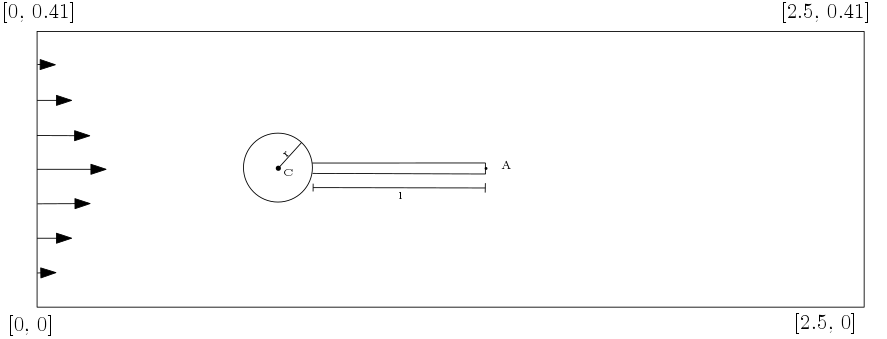
\includegraphics[scale=0.5]{./Fig/turekflag.png}
\end{figure}

Several quantites for comparion is presented in \cite{Hron2006} for validation purposes. We will report
\begin{itemize}
\item The position of point A(t) as the strucutre undergoes deformation.
\item Drag and lift forces exerted on of the whole interior geometry in contact with the fluid, consisting of the rigid circle and the elastic beam. 
\begin{align*}
(F_D, F_L) = \int_{\Gamma} \mathbf{\sigma} \cdot \mathbf{n} dS
\end{align*}
Where \textbf{n} is the unit normal vector, pointing into the fluid domain. 
\end{itemize}
The amplitude and mean values for the time dependent properties are calculated from the last period of oscillations, together with the period. 

\begin{table}[h]
\centering
\caption{Benchmark environment}
\label{my-label}
\begin{tabular}{ |p{3cm}||p{3cm}|p{3cm}|p{3cm}|  }
 \hline
 \multicolumn{4}{|c|}{Solid parameters} \\
 \hline
 parameter              & FSI1 & FSI2 & FSI3 \\
 \hline
 $\rho^s [10^{3} \frac{kg}{m^3}]$ & 1    & 10   & 1    \\
$\nu^s$ & 0.4  & 0.4  & 0.4  \\
$\mu^s  [10^{6}\frac{kg}{ms^2}]$  & 0.5  & 0.5  & 2.0  \\
 \hline
 \multicolumn{4}{|c|}{Fluid parameters} \\
 \hline
$\rho^f [10^{3}\frac{kg}{m^3}]$ & 1    & 1    & 1    \\
$\nu^f  [10^{-3}\frac{m^2}{s}]$  & 1    & 1    & 1    \\
U                      & 0.2  & 1    & 2    \\
parameter              & FSI1 & FSI2 & FSI3 \\
Re                     & 20   & 100  & 200 \\
\hline
\end{tabular}
\end{table}


\subsection{FSI1}
The first environment yields a steady state solution for the system. It is meant as a basic implementation test as it applies small deformations to the system. Therefore is provides a test for the solving procedure, but doesn't excess large constrain of choice of mesh extrapolation operator. 

\begin{table}[h!]
\centering
\caption{FSI 1}
\label{my-label}
\begin{tabular}{ |p{2.5cm}||p{1cm}|p{1cm}|p{2.3cm}|p{2.3cm}|p{1.2cm}|p{1.2cm}|}
 \hline
  \multicolumn{7}{|c|}{$\Delta t = 0.5$} \\
   \hline
 Model & nel & ndof & ux of A [x $10^{3}$]  &uy of A [x $10^{3}$]& Drag  & Lift \\
 \hline
Biharmonic bc2 & 1 &1 & 0.0228  &  0.7740  & 14.17280  &  0.7614 \\
 \hline
Biharmonic bc1 & 1 &1 & 0.0228 &   0.7737  & 14.17281 &  0.7612  \\
 \hline
Elastic        & 1 &1 & 0.0227  &  0.7960  & 14.17283 &  0.7607  \\
 \hline
Laplace        & 1 &1 & 0.0227  &  0.7958  & 14.17285 &  0.7607   \\
 \hline
  \multicolumn{7}{|c|}{$\Delta t = 0.1$} \\
   \hline
 Model & nel & ndof & ux of A [x $10^{3}$]  &uy of A [x $10^{3}$]& Drag  & Lift \\
 \hline
Biharmonic bc2 & 1 &1 & 0.0228 &  0.7743  & 14.17279 & 0.76162  \\
 \hline
Biharmonic bc1 & 1 &1 & 0.0228  &  0.7739 & 14.17280 & 0.76142 \\
 \hline
Elastic       & 1 &1 & 0.0228  &  0.7962  & 14.17281 & 0.76092 \\
 \hline
Laplace        & 1 &1 & 0.0228  & 0.7961  & 14.17284 & 0.76090 \\
\hline
\end{tabular}
\end{table}

\subsection{FSI2}
The second environment results in a periodic solution. It proved to be one of the most demanding tests due to its large deformation, leading to the risk of entangled mesh cells. As such this raised the need for a high quality extrapolation of the solid deformation.
\\
\subsection{FSI3}    
The final environment does not induce deformation to the extent of the FSI2 benchmark. However a critical phase in the transition to the periodic solution was discovered, where the pressure oscillation induces a large deformation to the system. 

\begin{table}[h!]
\centering
\caption{FSI 3}
\label{my-label}
\begin{tabular}{lllll}
 \hline
Test & x-comp A          & y-comp A             & drag                   & lift                 \\
 \hline
bc1 &                   &                      & 442.9 +/ 17.26         & 2.83 +- 148.8        \\
 \hline
bc2 &                   &                      & 442.8 +/ 17.44         & 3.06 +-147.9         \\
 \hline
Ref & 2.69  2.53  &   1.48  34.38 5.3   & 457. 22.66 10.9 & 2.22 149.78 5.3 \\
 \hline
\end{tabular}
\end{table}


\section{Mesh movement}
The final enviroment 
%\newpage

%\chapter{Application}
\section{Numericnerding eller applik ?}


\bibliographystyle{plain}
\bibliography{./Cite/Books,./Cite/ALECoupled,./Cite/Decoupled,./Cite/NavierStokes,./Cite/Verification,./Cite/EulerianFormulation,./Cite/Meshupdate}
\end{document}